\documentclass[10pt]{beamer}

% Theme and color scheme
\usetheme{metropolis}
%\usecolortheme{seahorse}
\setbeamertemplate{navigation symbols}{}
\setbeamertemplate{footline}[frame number]

% Packages
\usepackage{graphicx}
\usepackage{comment}
\usepackage{amsmath}
\usepackage{animate} % For animated sequences (requires viewer support)
\usepackage{tikz}
\usetikzlibrary{decorations.pathreplacing}
\usepackage{booktabs}
\usepackage{xcolor}
% \usepackage{subcaption} % Incompatible with beamer; not used

% Title page information
\title[The Grammar of Conflict]{The Grammar of Conflict}
\subtitle{Discovering Universal Patterns in Armed Violence}
\author[T. Chadefaux]{Thomas Chadefaux}
\institute[TCD]{Trinity College Dublin \\ Department of Political Science}
\date{\today}

% Custom commands
\newcommand{\highlight}[1]{\textcolor{red}{\textbf{#1}}}

\begin{document}

% ====================
% TITLE SLIDE
% ====================
\begin{frame}
% Background image with transparency
\begin{tikzpicture}[remember picture,overlay]
\node[at=(current page.center), opacity=0.15] {
  \includegraphics[width=0.5\paperwidth,height=0.5\paperheight,keepaspectratio]{../extracted_media/Chadefaux_Berlin2025_2/ppt/media/image5.png}
};
\end{tikzpicture}

\begin{columns}[T]
\begin{column}{0.75\textwidth}
\titlepage
\end{column}
\begin{column}{0.25\textwidth}
\vspace{1cm}
\begin{center}
\includegraphics[width=0.8\textwidth]{../extracted_media/Chadefaux_Berlin2025_2/ppt/media/image4.jpeg}\\[0.3cm]
\includegraphics[width=0.8\textwidth]{../extracted_media/Chadefaux_Berlin2025_2/ppt/media/image6.png}\\[0.3cm]
\includegraphics[width=0.8\textwidth]{../extracted_media/Chadefaux_Berlin2025_2/ppt/media/image7.png}
\end{center}
\end{column}
\end{columns}
\note[item]{Welcome - 45 minute presentation on the Patterns of Conflict Emergence (PaCE) research program}
\note[item]{This work bridges conflict studies, time series analysis, and pattern recognition}
\note[item]{Aimed at showing statisticians why temporal patterns in conflict data matter}
\note[item]{Will cover: data challenges, methodological innovations, empirical results}
\end{frame}


\begin{frame}{Dublin 1922}
\includegraphics[width=\textwidth]{Figs/dublin1922.png}
\end{frame}


\begin{frame}{Dublin 2025}
\includegraphics[width=\textwidth]{Figs/dublin2024.png}
\end{frame}
% ====================
% PART 1: THE DOMAIN & DATA
% ====================


\begin{frame}{We all like stories}
%\begin{columns}
%\begin{column}{0.5\textwidth}

\begin{columns}
\begin{column}{0.5\textwidth}
\begin{figure}
\includegraphics[width=0.9\linewidth]{Figs/tragedy.png} 
\caption{Tragedy}
\end{figure}
\end{column}
%
\begin{column}{0.5\textwidth}
\begin{figure}
\includegraphics[width=0.9\linewidth]{Figs/starWars.png} 
\caption{Seven Point Story}
\end{figure}
\end{column}
%\end{column}
\end{columns}
\end{frame}






\begin{frame}{Financial analysts like stories}
\begin{figure}
\centering
\includegraphics[height=\textheight]{Figs/financePatterns.png}
\end{figure}
\end{frame}


\begin{frame}{Doctors like stories}
\begin{figure}
\centering
\includegraphics[height=\textheight]{Figs/doctorsPatterns.png}
\end{figure}
\end{frame}

\begin{frame}{Qualitative social scientists like stories}
\begin{figure}
\centering
\includegraphics[width=\textwidth]{Figs/qualitativePatterns.png}
\end{figure}
\end{frame}


\begin{frame}{Theorists likes stories}
\begin{figure}
\centering
\includegraphics[width=\textwidth]{Figs/theoristsPatterns.png}
\end{figure}
\end{frame}


\begin{frame}{Conflict researchers DO NOT like stories}
\begin{columns}
\begin{column}{0.5\textwidth}
%
\begin{figure}
\centering
\includegraphics[width=\linewidth]{Figs/quantativeStories1.png}
\end{figure}
\end{column}
\begin{column}{0.5\textwidth}
\end{column}
\end{columns}
\end{frame}

\begin{frame}{Conflict researchers DO NOT like stories}
\begin{columns}
\begin{column}{0.5\textwidth}
%
\begin{figure}
\centering
\includegraphics[width=\linewidth]{Figs/quantativeStories2.png}
\end{figure}
\end{column}
\begin{column}{0.5\textwidth}
\end{column}
\end{columns}
\end{frame}

\begin{frame}{Conflict researchers DO NOT like stories}
\begin{columns}
\begin{column}{0.5\textwidth}
%
\begin{figure}
\centering
\includegraphics[width=\linewidth]{Figs/quantativeStories2.png}
\end{figure}
\end{column}
\begin{column}{0.5\textwidth}
\begin{figure}
\centering
\includegraphics[width=\linewidth]{Figs/quantativeStories3.png}
\end{figure}
\vfill
\end{column}
\end{columns}
\end{frame}



\begin{frame}{Conflict researchers DO NOT like stories}
\begin{columns}
\begin{column}{0.5\textwidth}
%
\begin{figure}
\centering
\includegraphics[width=\linewidth]{Figs/quantativeStories2.png}
\end{figure}
\end{column}
\begin{column}{0.5\textwidth}
\begin{figure}
\centering
\includegraphics[width=\linewidth]{Figs/quantativeStories4.png}
\end{figure}
\vfill
\end{column}
\end{columns}
\end{frame}




% ====================
% PART 3: WHY PATTERNS EMERGE
% ====================

\section{Why patterns (might) emerge}

\begin{frame}{The Grammar Hypothesis}
\begin{center}
\Large
Hypothesis: Armed conflicts follow systematic temporal patterns
\end{center}

\vspace{1cm}

\begin{columns}
\begin{column}{0.5\textwidth}
\textbf{Language Grammar}
\begin{itemize}
\item Universal rules constrain word order
\item Limited set of sentence structures
\item Surface variation, deep structure
\item Predictable patterns
\end{itemize}
\end{column}
\begin{column}{0.5\textwidth}
\textbf{Conflict Grammar}
\begin{itemize}
\item Universal rules constrain event sequences
\item Limited set of trajectory types
\item Surface variation, deep structure
\item Predictable patterns
\end{itemize}
\end{column}
\end{columns}

\note[item]{Central hypothesis: Conflicts have a "grammar"}
\note[item]{Not claiming conflicts ARE language, but similar structure}
\note[item]{Language analogy: Universal grammar (Chomsky) - deep structure}
\note[item]{Many languages, but shared deep principles}
\note[item]{Similarly: Many conflicts, but shared temporal principles}
\note[item]{Question: Why would conflicts follow patterns at all?}
\note[item]{Three mechanisms explain this...}
\end{frame}

\begin{frame}{Mechanism 1: Patterns from Simple Rules}
Complex dynamics can emerge from simple differential equations

\begin{columns}
\begin{column}{0.5\textwidth}
\textbf{Toy Model}
\begin{align*}
\frac{dp}{dt} &= \alpha p - \beta p v \\
\frac{dv}{dt} &= \delta pv - \gamma v
\end{align*}

\begin{itemize}
\item $p$: Civilian population
\item $v$: Violence intensity
\item Violence $\uparrow$ when population $\uparrow$
\item Population $\downarrow$ when violence $\uparrow$ (displacement)
\end{itemize}
\end{column}
\begin{column}{0.5\textwidth}
\begin{center}
\includegraphics[width=0.9\textwidth]{Figs/lotke.pdf}

\small Predator-prey dynamics\\
generate cycles
\end{center}
\end{column}
\end{columns}


\note[item]{First mechanism: Spontaneous pattern formation}
\note[item]{Borrowed from ecology: Lotka-Volterra equations}
\note[item]{Obviously oversimplified for conflict! But illustrative}
\note[item]{Basic feedback: More people $\rightarrow$ more violence possible}
\note[item]{But violence $\rightarrow$ people flee $\rightarrow$ less violence}
\note[item]{This creates oscillations, cycles}
\note[item]{Real conflicts have many more feedbacks: mobilization, resources, fatigue}
\note[item]{Point: Don't need complicated story for patterns to emerge}
\note[item]{Simple nonlinear dynamics $\rightarrow$ rich temporal structure}
\note[item]{Analogy: Physical systems (waves, turbulence), biological (heartbeat, neurons)}
\end{frame}

\begin{frame}{Mechanism 2: Patterns in Driving Variables}
If causal variables follow patterns, so will outcomes

\begin{columns}
\begin{column}{0.5\textwidth}
\textbf{Structured Drivers}
\begin{itemize}
\item \textbf{Economic cycles}: Harvest seasons, commodity prices
\item \textbf{Political cycles}: Elections, budget cycles
\item \textbf{Climate cycles}: Rainy/dry seasons
\item \textbf{Resource cycles}: Mobilization/exhaustion
\end{itemize}

\vspace{0.3cm}

These combine to create \highlight{complex temporal structures} in conflict
\end{column}
\begin{column}{0.5\textwidth}
\begin{center}
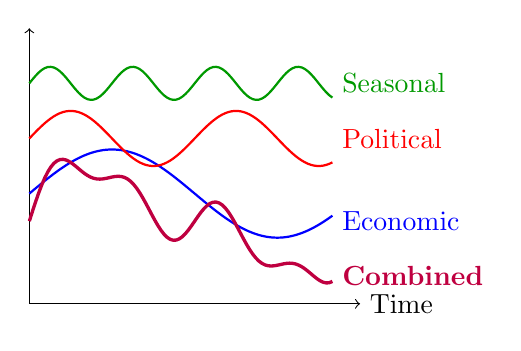
\begin{tikzpicture}[scale=0.7]
% Show multiple cycles combining
\draw[->] (0,0) -- (6,0) node[right] {Time};
\draw[->] (0,0) -- (0,5);

% Economic cycle (slow)
\draw[blue, thick, domain=0:5.5, samples=100] plot (\x, {2 + 0.8*sin(\x*60)});
\node[blue, right] at (5.5,1.5) {Economic};

% Political cycle (medium)
\draw[red, thick, domain=0:5.5, samples=100] plot (\x, {3 + 0.5*sin(\x*120)});
\node[red, right] at (5.5,3) {Political};

% Seasonal cycle (fast)
\draw[green!60!black, thick, domain=0:5.5, samples=100] plot (\x, {4 + 0.3*sin(\x*240)});
\node[green!60!black, right] at (5.5,4) {Seasonal};

% Combined
\draw[purple, very thick, domain=0:5.5, samples=100] plot (\x, {1.5 + 0.8*sin(\x*60) + 0.5*sin(\x*120) + 0.3*sin(\x*240)});
\node[purple, right] at (5.5,0.5) {\textbf{Combined}};
\end{tikzpicture}
\end{center}
\end{column}
\end{columns}

\note[item]{Second mechanism: Structure in driving variables}
\note[item]{If causes have temporal patterns, effects will too}
\note[item]{Economic: Agricultural cycles affect food security, grievances}
\note[item]{Political: Electoral cycles create windows for repression/resistance}
\note[item]{Climate: Dry season $\rightarrow$ easier to move troops; rainy $\rightarrow$ pause}
\note[item]{Resource: Rebels need time to rearm, recruit after battle}
\note[item]{These cycles interact: Multiple time scales}
\note[item]{Creates complex but structured temporal patterns}
\note[item]{Standard lags (t-1, t-2) can't capture this complexity}
\note[item]{But pattern recognition can detect combined signatures}
\end{frame}

\begin{frame}{Mechanism 3: Strategic Adaptation}
Actors detect patterns and respond to them

\begin{columns}
\begin{column}{0.5\textwidth}

\begin{itemize}
\item Humans excel at pattern recognition
\item Build mental models of sequences
\item Make decisions based on perceived trends
\item Anticipate opponent behavior
\end{itemize}
\end{column}
\begin{column}{0.5\textwidth}
\textbf{Example: Tit-for-Tat}

\begin{center}
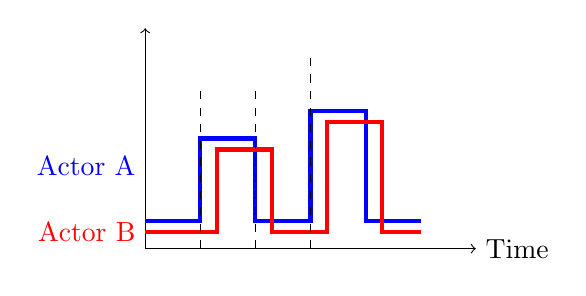
\begin{tikzpicture}[scale=0.7]
\draw[->] (0,0) -- (6,0) node[right] {Time};
\draw[->] (0,0) -- (0,4);

% Actor A (blue)
\draw[blue, thick, line width=1.5pt] (0,0.5) -- (1,0.5) -- (1,2) -- (2,2) -- (2,0.5) -- (3,0.5) -- (3,2.5) -- (4,2.5) -- (4,0.5) -- (5,0.5);
\node[blue, left] at (0,1.5) {Actor A};

% Actor B (red) - responds with delay
\draw[red, thick, line width=1.5pt] (0,0.3) -- (1.3,0.3) -- (1.3,1.8) -- (2.3,1.8) -- (2.3,0.3) -- (3.3,0.3) -- (3.3,2.3) -- (4.3,2.3) -- (4.3,0.3) -- (5,0.3);
\node[red, left] at (0,0.3) {Actor B};

\draw[dashed] (1,0) -- (1,3);
\draw[dashed] (2,0) -- (2,3);
\draw[dashed] (3,0) -- (3,3.5);
\end{tikzpicture}
\end{center}

Action-reaction cycles\\create patterns
\end{column}
\end{columns}

\note[item]{Third mechanism: Strategic adaptation by actors}
\note[item]{This is the most social science explanation}
\note[item]{Conflict actors aren't blind - they observe and adapt}
\note[item]{If government escalating, rebels preempt or flee}
\note[item]{If rebels pause (regroup), government may intensify}
\note[item]{Creates action-reaction cycles}
\note[item]{These are self-reinforcing: patterns create patterns}
\note[item]{Example: If violence always surges in dry season, both sides prepare for it}
\note[item]{This coordination creates predictable cycles}
\note[item]{Related to game theory: Repeated games, learning}
\end{frame}

\begin{frame}{Evidence: How People Process Conflict Sequences}
\textbf{Experimental findings} (Han \& Chadefaux 2026): People evaluate diplomatic sequences

\begin{columns}
\begin{column}{0.5\textwidth}
\textbf{Three Temporal Dimensions}
\begin{enumerate}
\item \textbf{Direction}: Cooperation increasing or decreasing?
\item \textbf{Consistency}: Regular or erratic progression?
\item \textbf{Acceleration}: Speeding up or slowing down?
\end{enumerate}

\vspace{0.3cm}

People construct \highlight{narratives} from event sequences
\end{column}
\begin{column}{0.5\textwidth}
\begin{center}
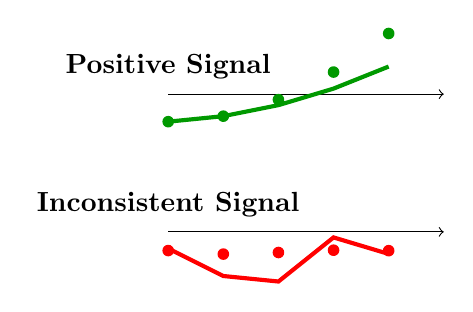
\begin{tikzpicture}[scale=0.7]
% Good pattern: increasing, consistent
\node at (0,4) {\textbf{Positive Signal}};
\draw[->] (0,3.5) -- (5,3.5);
\draw[thick, green!60!black, line width=1.5pt] (0,3) -- (1,3.1) -- (2,3.3) -- (3,3.6) -- (4,4);
\foreach \x in {0,1,2,3,4} {
    \fill[green!60!black] (\x,{3+0.1*\x*\x}) circle (3pt);
}

% Bad pattern: inconsistent
\node at (0,1.5) {\textbf{Inconsistent Signal}};
\draw[->] (0,1) -- (5,1);
\draw[thick, red, line width=1.5pt] (0,0.7) -- (1,0.2) -- (2,0.1) -- (3,0.9) -- (4,0.6);
\foreach \x in {0,1,2,3,4} {
    \fill[red] (\x,{0.5+0.2*rnd}) circle (3pt);
}
\end{tikzpicture}
\end{center}

Consistent increasing cooperation $\rightarrow$ trust

Inconsistent $\rightarrow$ skepticism
\end{column}
\end{columns}


\note[item]{Direct evidence that people process temporal patterns}
\note[item]{Experiments on US-China relations: Show people sequences of cooperative events}
\note[item]{People don't evaluate each event independently}
\note[item]{They construct narratives: "Things are getting better" vs "erratic"}
\note[item]{Three features matter: Direction, Consistency, Acceleration}
\note[item]{Increasing cooperation $\rightarrow$ optimism about future}
\note[item]{Inconsistent cooperation $\rightarrow$ skepticism even if overall positive}
\note[item]{This is "emplotment" - weaving events into stories}
\note[item]{If people think this way about cooperation, likely also about conflict}
\note[item]{Validates: Pattern recognition is how humans process political sequences}
\note[item]{Micro-foundation for macro-level patterns}
\end{frame}


%-------------------
%.       UNDERSTANDING CONFLICT DATA
%-------------------


\section{Conflict Data}

\begin{frame}{What Are We Measuring?}
\begin{columns}
\begin{column}{0.5\textwidth}
\textbf{Armed Conflict Events}
\begin{itemize}
\item Organized violence between actors
\item \emph{Predict: Battle-related deaths}
\item Georeferenced incidents
\item Daily/monthly aggregation
\end{itemize}

\vspace{0.5cm}

\textbf{Data Sources}
\begin{itemize}
\item Uppsala Conflict Data Program (UCDP)
\item 1989--2025 (36 years)
\item Global coverage
\item Updated monthly
\end{itemize}
\end{column}
\begin{column}{0.5\textwidth}
\begin{center}
\textbf{Example: Event Record}
\vspace{0.3cm}

\small
\begin{tabular}{ll}
\toprule
\textbf{Field} & \textbf{Value} \\
\midrule
Date & 2015-03-12 \\
Country & Syria \\
Location & Aleppo (36.2$\circ$N, 37.1$\circ$E) \\
Fatalities & 47 \\
Actor 1 & Government \\
Actor 2 & Rebel group \\
\bottomrule
\end{tabular}
\end{center}
\end{column}
\end{columns}

\note[item]{Start concrete: What exactly is a "conflict event"?}
\note[item]{UCDP codes organized violence with at least 1 fatality}
\note[item]{Georeferenced = we know where and when}
\note[item]{This is structured data, not unstructured news text}
\note[item]{Gold standard = most widely used, extensively validated}
\note[item]{Key point: We aggregate these events into time series}
\end{frame}


\begin{frame}{Sample Trajectories: Three Countries}
\begin{center}
% Placeholder for real time series from 3 countries showing different patterns
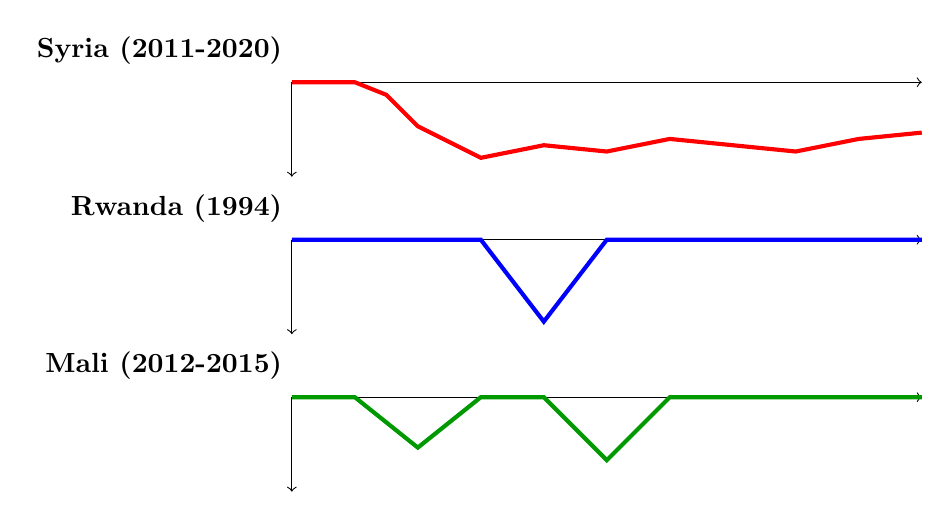
\begin{tikzpicture}[scale=0.8]
% Syria - sustained high intensity
\node[left] at (0,5) {\textbf{Syria (2011-2020)}};
\draw[->] (0,4.5) -- (10,4.5);
\draw[->] (0,4.5) -- (0,3);
\draw[thick, red, line width=1.5pt] (0,4.5) -- (1,4.5) -- (1.5,4.3) -- (2,3.8) -- (3,3.3) -- (4,3.5) -- (5,3.4) -- (6,3.6) -- (7,3.5) -- (8,3.4) -- (9,3.6) -- (10,3.7);

% Rwanda - sharp spike
\node[left] at (0,2.5) {\textbf{Rwanda (1994)}};
\draw[->] (0,2) -- (10,2);
\draw[->] (0,2) -- (0,0.5);
\draw[thick, blue, line width=1.5pt] (0,2) -- (2,2) -- (3,2) -- (4,0.7) -- (5,2) -- (10,2);

% Mali - episodic
\node[left] at (0,0) {\textbf{Mali (2012-2015)}};
\draw[->] (0,-0.5) -- (10,-0.5);
\draw[->] (0,-0.5) -- (0,-2);
\draw[thick, green!60!black, line width=1.5pt] (0,-0.5) -- (1,-0.5) -- (2,-1.3) -- (3,-0.5) -- (4,-0.5) -- (5,-1.5) -- (6,-0.5) -- (7,-0.5) -- (10,-0.5);
\end{tikzpicture}
\end{center}

\textbf{Different conflict profiles}: Sustained, spike, episodic

\note[item]{Show heterogeneity in the data}
\note[item]{Syria: Long, sustained civil war with persistent high fatalities}
\note[item]{Rwanda: Genocide - massive spike then rapid end}
\note[item]{Mali: Episodic violence with multiple flare-ups}
\note[item]{Challenge: How do we model processes this diverse?}
\note[item]{Traditional approach: Focus on covariates (GDP, regime type, etc.)}
\note[item]{Our approach: Focus on temporal shapes}
\end{frame}




\begin{frame}{Aggregation: Country- vs Grid-level}
\begin{figure}
\includegraphics[height=0.4\textheight]{Figs/countryLevel.png}
\end{figure}
\begin{figure}
\includegraphics[height=0.4\textheight]{Figs/prioLevel.png}
\end{figure}

\end{frame}



\begin{frame}{Zero Inflation}
\begin{columns}
\begin{column}{0.5\textwidth}
\textbf{The Problem}
\begin{itemize}
\item Most country-months: \highlight{zero fatalities}
\item Distribution extremely skewed
\end{itemize}

\end{column}
%
%
\begin{column}{0.5\textwidth}
\includegraphics[height=0.5\textheight]{Figs/skew1.pdf}\\
\includegraphics[height=0.5\textheight]{Figs/skew2.pdf}
\end{column}
\end{columns}

\note[item]{Critical data feature: Extreme zero-inflation}
\note[item]{Typically 80-90\% of country-months have zero fatalities}
\note[item]{This is actually good news (most places peaceful most of the time)}
\note[item]{But statistically challenging: bulk of data at boundary}
\note[item]{Question: How do we model this? Two-part model? Zero-inflated Poisson?}
\note[item]{Our approach: Filter to conflict-active periods OR normalize patterns}
\note[item]{Focus on shape during active periods, not levels including zeros}
\end{frame}



%
%\begin{frame}{Zero Inflation}
%\begin{columns}
%\begin{column}{0.5\textwidth}
%\includegraphics[width=\textwidth]{Figs/distPRIO.png}\\
%\begin{center}\small All conflict data\end{center}
%\end{column}
%\begin{column}{0.5\textwidth}
%\includegraphics[width=\textwidth]{Figs/distStateLevel.png}
%\begin{center}\small Filtered (active periods only)\end{center}
%\end{column}
%\end{columns}
%
%\vspace{0.3cm}
%
%\note[item]{Left: Including all peaceful periods - dominated by flat zero patterns}
%\note[item]{Right: Filter to windows with at least some violence - reveals structure}
%\note[item]{This is analogous to analyzing active periods in other domains}
%\note[item]{We're not predicting onset from peace (different problem)}
%\note[item]{We're predicting trajectories once violence has started}
%\note[item]{Both are important, but different statistical problems}
%\end{frame}


\begin{frame}{Heterogeneity}
\begin{columns}
\begin{column}{0.5\textwidth}
\begin{itemize}
\item Small civil wars: 10s of deaths/year
\item Major conflicts: 10,000s of deaths/month
\item \highlight{Orders of magnitude difference}
\item Heavy-tailed distribution

\end{itemize}

\end{column}
\begin{column}{0.5\textwidth}
\begin{center}
\begin{figure}
\includegraphics[width=\textwidth]{Figs/sandpilesCederman.png}
\caption{Source: Cederman 2003}
\end{figure}
\end{center}

\vspace{0.3cm}
\textbf{Power law}: $P(X > x) \sim x^{-\alpha}$
\end{column}
\end{columns}

\textbf{Our solution}: \highlight{Min-max normalization} within subsequences

\note[item]{Third challenge: Massive heterogeneity in scale}
\note[item]{Small conflicts in Burundi vs Syria - 3-4 orders of magnitude difference}
\note[item]{Distribution is heavy-tailed, possibly power law}
\note[item]{Can't just pool all countries together and estimate one model}
\note[item]{But we want to find patterns that generalize across conflicts}
\note[item]{Solution: Normalize each subsequence to [0,1] range}
\note[item]{Now comparing shapes, not absolute levels}
\note[item]{A spike from 10$\rightarrow$100 deaths has same shape as 1000$\rightarrow$10000}
\note[item]{This is key to finding universal patterns}
\end{frame}

\begin{frame}{Measurement Issues}
\begin{columns}
\begin{column}{0.5\textwidth}
\textbf{Reporting Bias}
\begin{itemize}
\item Remote areas: under-reported
\item Media attention varies
\item Government censorship
\end{itemize}

\vspace{0.5cm}

\textbf{Temporal Variation}
\begin{itemize}
\item Data quality improves over time
\item Cell phones, social media increase reporting
\item 1990s data sparser than 2010s
\end{itemize}
\end{column}
\begin{column}{0.5\textwidth}
\textbf{Spatial Variation}
\begin{itemize}
\item Syria: heavily documented
\item Central African Republic: less coverage
\item Urban vs rural differences
\end{itemize}


\end{column}
\end{columns}

\note[item]{Fourth issue: Measurement error and bias}
\note[item]{UCDP is best available, but not perfect}
\note[item]{Remote conflicts (DRC forests) vs urban (Aleppo) - different coverage}
\note[item]{Data quality improves: 2010s better than 1990s (cell phones, social media)}
\note[item]{Could this create spurious patterns? Maybe!}
\note[item]{That's why we test extensively: across decades, regions, scales}
\note[item]{If patterns appear in both 1990s Africa and 2010s Middle East $\rightarrow$ probably real}
\note[item]{If only in recent high-quality data $\rightarrow$ might be artifact}
\note[item]{Spoiler: patterns are robust, suggesting they're real}
\end{frame}


% ====================
% PART 2: THE FORECASTING PROBLEM
% ====================

\section{The Forecasting Problem}

\begin{frame}{Traditional Approach: Structural Covariates}
\begin{columns}
\begin{column}{0.5\textwidth}
\textbf{The Standard Model}
\begin{itemize}
\item Economic: GDP, inequality, resources
\item Political: Regime type, institutions
\item Demographic: Population, youth bulge
\item Social: Ethnic fractionalization
\item Historical: Past conflict
\end{itemize}

\vspace{0.3cm}

\textbf{Examples}
\begin{itemize}
\item Goldstone et al. (2010)
\item Hegre et al. (2013)
\item ViEWS System
\end{itemize}
\end{column}
\begin{column}{0.5\textwidth}
\begin{center}
\textbf{Regression Framework}

\vspace{0.5cm}

$\Pr(\text{Conflict}_{i,t}) = f($
\begin{itemize}
\item[] GDP$_{i,t}$
\item[] Democracy$_{i,t}$
\item[] Population$_{i,t}$
\item[] Neighbors$_{i,t}$
\item[] History$_{i,t-1}$
\item[] $\ldots$
\end{itemize}
$)$

\vspace{0.5cm}

Often 20-50+ covariates
\end{center}
\end{column}
\end{columns}

\note[item]{Traditional conflict forecasting: structural risk factors}
\note[item]{Logic: Poor, weak, divided countries are at risk}
\note[item]{Cross-sectional variation: Why Syria vs Switzerland?}
\note[item]{Large regression models with many covariates}
\note[item]{These models work! They identify at-risk countries}
\note[item]{Major research programs: Political Instability Task Force, ViEWS}
\note[item]{But there's a problem...}
\end{frame}


\begin{frame}{Yet, adding covariates does not really improve forecasts}
\begin{center}
\includegraphics[width=0.7\textwidth]{Figs/RMSE.png}
\end{center}

 AR $\approx$ AR+Cov $>>$ Cov

$\rightarrow$Temporal information is more predictive than structural covariates

(source: Schincariol \& Chadefaux 2026)

\note[item]{Shocking result from our EPJ Data Science paper}
\note[item]{Compare three models: (1) Autoregressive only, (2) Covariates only, (3) Both}
\note[item]{AR model: Just uses past fatalities, no covariates}
\note[item]{Cov model: Uses GDP, regime, population, etc. - no past fatalities}
\note[item]{AR+Cov: Uses both}
\note[item]{Result: AR alone performs nearly as well as AR+Cov!}
\note[item]{Both massively outperform Cov alone}
\note[item]{This is counterintuitive - decades of research on covariates}
\note[item]{But: temporal patterns contain the information}
\note[item]{Covariates help, but marginal improvement is small}
\note[item]{This validates focusing on temporal structure}
\end{frame}

% ====================
% PART 4: METHODS
% ====================

\section{Methods}

\begin{frame}{Preprocessing: Windows and Normalization}
\begin{columns}
\begin{column}{0.49\textwidth}
\textbf{Windowing}
\begin{itemize}
\item Divide each time series into subsequences
\item Length $w$ = 12, 24, or 36 months
\item {Overlapping}: Slide by 1 month
\item Each window is a potential pattern
\end{itemize}
\vfill

\end{column}
\begin{column}{0.49\textwidth}

\textbf{Normalization}
\begin{itemize}
\item Within each window: Min-max scale
\item $x_i' = \frac{x_i - \min(x)}{\max(x) - \min(x)}$
\item Maps to [0, 1]
\item Preserves shape, removes scale
\end{itemize}
\vspace{0.3cm}

\begin{center}
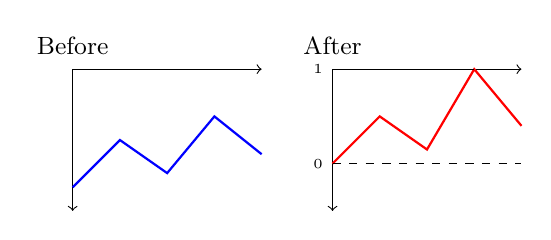
\begin{tikzpicture}[scale=0.6]
% Before normalization
\node at (0,3.5) {\small Before};
\draw[->] (0,3) -- (4,3);
\draw[->] (0,3) -- (0,0);
\draw[thick, blue] (0,0.5) -- (1,1.5) -- (2,0.8) -- (3,2) -- (4,1.2);

% After normalization
\node at (5.5,3.5) {\small After};
\draw[->] (5.5,3) -- (9.5,3);
\draw[->] (5.5,3) -- (5.5,0);
\draw[thick, red] (5.5,1) -- (6.5,2) -- (7.5,1.3) -- (8.5,3) -- (9.5,1.8);
\draw[dashed] (5.5,3) -- (9.5,3);
\draw[dashed] (5.5,1) -- (9.5,1);
\node[left] at (5.5,3) {\tiny 1};
\node[left] at (5.5,1) {\tiny 0};
\end{tikzpicture}
\end{center}
\end{column}
\end{columns}

\note[item]{First steps: Windowing and normalization}
\note[item]{Windowing: Divide 10-year series into 12-month chunks}
\note[item]{Why overlap? Escalation might start in March not January}
\note[item]{Sliding window captures all possible starting points}
\note[item]{Cost: Creates dependence between windows - but worth it}
\note[item]{Normalization: Critical for comparing across conflicts}
\note[item]{10$\rightarrow$100 deaths has same shape as 1000$\rightarrow$10000}
\note[item]{Min-max preserves relative dynamics, removes absolute scale}
\note[item]{Now can compare Syrian and Malian conflicts despite magnitude differences}
\end{frame}

\begin{frame}{Comparing Sequences: Dynamic Time Warping (DTW)}
\textbf{Problem}: Standard distance metrics (Euclidean, correlation) assume alignment
\begin{figure}
\centering
\includegraphics[height=0.8\textheight]{Figs/dtw.jpg}
\end{figure}
\note[item]{Key innovation: Dynamic Time Warping}
\note[item]{Problem: Same pattern at different speeds looks different}
\note[item]{Example: Escalation in 6 months vs 9 months}
\note[item]{Euclidean distance: Point-to-point comparison}
\note[item]{Escalation at month 3 compared to observation at month 3}
\note[item]{If real escalation happens at month 4, mismatch!}
\note[item]{DTW: Find best alignment, allow warping}
\note[item]{Can map month 3 of series 1 to month 4 of series 2}
\note[item]{Constraint: Must be monotonic (time can't go backwards)}
\note[item]{Figure shows: Two similar escalations, aligned despite speed differences}
\note[item]{This is why we can find patterns across diverse conflicts}
\end{frame}


\begin{frame}{Shape Finder: The Input Sequence}
\textbf{What we're trying to forecast}

\begin{columns}
\begin{column}{0.39\textwidth}
\textbf{Input = Recent Trajectory}
\begin{itemize}
\item Last 10 months of fatalities
\item Example: Afghanistan Mar--Dec 2021
\item This is the \textit{shape} we'll match
\end{itemize}

\vspace{0.5cm}

\textbf{Goal}
\begin{itemize}
\item Predict next 12 months (2022)
\item Find: What happened after similar patterns historically?
\end{itemize}
\end{column}
\begin{column}{0.59\textwidth}
\begin{center}
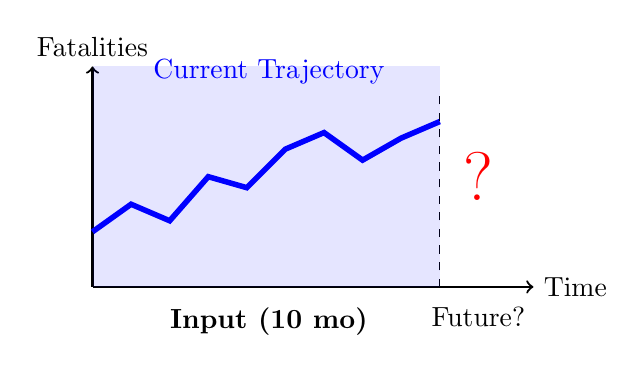
\begin{tikzpicture}[scale=0.7]
% Time axis
\draw[->, thick] (0,0) -- (8,0) node[right] {Time};
\draw[->, thick] (0,0) -- (0,4) node[above] {Fatalities};

% Input sequence (10 months)
\draw[blue, very thick, line width=2pt] (0,1) -- (0.7,1.5) -- (1.4,1.2) -- (2.1,2) -- (2.8,1.8) -- (3.5,2.5) -- (4.2,2.8) -- (4.9,2.3) -- (5.6,2.7) -- (6.3,3);

% Mark input period
\draw[dashed] (6.3,0) -- (6.3,3.5);
\node[below] at (3.2,-0.2) {\textbf{Input (10 mo)}};
\node[below] at (7,-0.2) {Future?};

% Highlight input
\fill[blue, opacity=0.1] (0,0) rectangle (6.3,4);

% Question mark for future
\node[font=\Huge, color=red] at (7,2) {?};

% Labels
\node[above, blue] at (3.2,3.5) {Current Trajectory};
\end{tikzpicture}
\end{center}
\end{column}
\end{columns}

\note[item]{First: Define what we're working with}
\note[item]{Input is recent 10-month fatality trajectory}
\note[item]{Example: Afghanistan January through October 2021}
\note[item]{This shows recent trend: escalating, stable, or de-escalating}
\note[item]{Goal: Forecast what happens in next 12 months}
\note[item]{Method: Find similar historical trajectories, see what happened next}
\note[item]{This is autoregressive - uses only past fatalities}
\note[item]{No covariates needed (GDP, regime type, etc.)}
\end{frame}

\begin{frame}{Shape Finder: Building the Historical Repository}
\textbf{Creating a library of all possible patterns}

\begin{center}
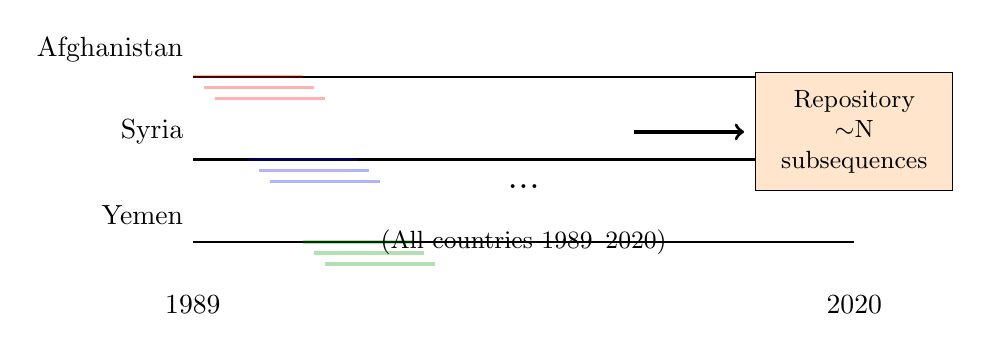
\begin{tikzpicture}[scale=0.7]
% Afghanistan timeline
\node[left] at (0,4) {Afghanistan};
\draw[thick] (0,3.5) -- (12,3.5);
\draw[red, very thick, opacity=0.3] (0,3.5) -- (2,3.5);
\draw[red, very thick, opacity=0.3] (0.2,3.3) -- (2.2,3.3);
\draw[red, very thick, opacity=0.3] (0.4,3.1) -- (2.4,3.1);

% Syria timeline
\node[left] at (0,2.5) {Syria};
\draw[thick] (0,2) -- (12,2);
\draw[blue, very thick, opacity=0.3] (1,2) -- (3,2);
\draw[blue, very thick, opacity=0.3] (1.2,1.8) -- (3.2,1.8);
\draw[blue, very thick, opacity=0.3] (1.4,1.6) -- (3.4,1.6);

% Yemen timeline
\node[left] at (0,1) {Yemen};
\draw[thick] (0,0.5) -- (12,0.5);
\draw[green!60!black, very thick, opacity=0.3] (2,0.5) -- (4,0.5);
\draw[green!60!black, very thick, opacity=0.3] (2.2,0.3) -- (4.2,0.3);
\draw[green!60!black, very thick, opacity=0.3] (2.4,0.1) -- (4.4,0.1);

% Ellipsis
\node at (6,1.5) {\Large ...};
\node[font=\small] at (6,0.5) {(All countries 1989--2020)};

% Time labels
\node[below] at (0,-0.3) {1989};
\node[below] at (12,-0.3) {2020};

% Arrow to repository
\draw[->, very thick] (8,2.5) -- (10,2.5);
\node[draw, rectangle, fill=orange!20, minimum width=2.5cm, minimum height=1.5cm, align=center, font=\small] at (12,2.5) {Repository\\$\sim$N\\subsequences};
\end{tikzpicture}
\end{center}

\vspace{0.2cm}

\textbf{Key features}:
\begin{itemize}
\item \textbf{Rolling windows}: Overlapping 10-month subsequences
\item \textbf{Flexibility}: Windows 8--12 months (captures different speeds)
\item \textbf{Comprehensive}: Every country, every month, 1989--2020
\end{itemize}

\note[item]{Step 1: Build comprehensive historical repository}
\note[item]{Take every country's fatality time series from 1989-2020}
\note[item]{Partition into overlapping 10-month windows}
\note[item]{Rolling window: Jan-Oct, Feb-Nov, Mar-Dec, etc.}
\note[item]{Why overlapping? Patterns might start mid-year}
\note[item]{Window flexibility: Allow 8-12 months to match different speeds}
\note[item]{Syria escalation might take 6 months, Yemen 12 months}
\note[item]{Both should match if shape is similar}
\note[item]{Result: ~100,000 historical subsequences}
\note[item]{This is our reference library of conflict trajectories}
\end{frame}

\begin{frame}{Shape Finder: Finding Similar Patterns (DTW)}
\textbf{Which historical cases look like the current situation?}

\begin{columns}
\begin{column}{0.48\textwidth}
\textbf{Comparison Method: DTW}
\begin{itemize}
\item Compare input to all N subsequences
\item DTW distance measures similarity
\item Accounts for speed differences
\item Focuses on \textit{shape}, not scale
\end{itemize}

\vspace{0.3cm}

\textbf{Adaptive Filtering}
\begin{itemize}
\item Keep only similar matches
\item Threshold: Start at 0.1, increase until $\geq$ 5 matches
\item Typically find 15--30 analogues
\item Result: $p_{\text{filtered}}$
\end{itemize}
\end{column}
\begin{column}{0.48\textwidth}
\begin{center}
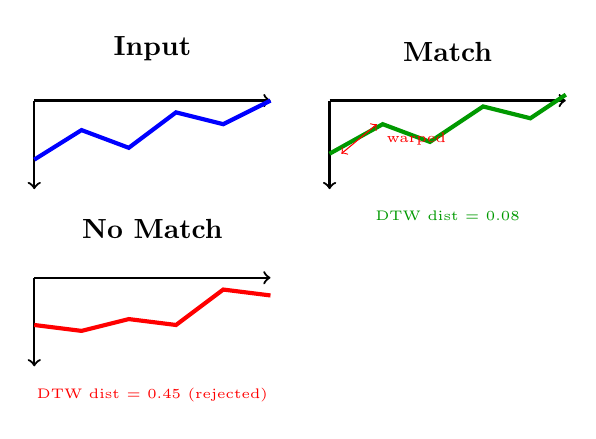
\begin{tikzpicture}[scale=0.75]
% Input pattern
\node[above] at (2,4.5) {\textbf{Input}};
\draw[->, thick] (0,4) -- (4,4);
\draw[->, thick] (0,4) -- (0,2.5);
\draw[blue, very thick, line width=1.5pt] (0,3) -- (0.8,3.5) -- (1.6,3.2) -- (2.4,3.8) -- (3.2,3.6) -- (4,4);

% Similar match
\node[above] at (7,4.5) {\textbf{Match}};
\draw[->, thick] (5,4) -- (9,4);
\draw[->, thick] (5,4) -- (5,2.5);
\draw[green!60!black, very thick, line width=1.5pt] (5,3.1) -- (5.9,3.6) -- (6.7,3.3) -- (7.6,3.9) -- (8.4,3.7) -- (9,4.1);
\node[below, font=\tiny, green!60!black] at (7,2.3) {DTW dist = 0.08};
\draw[<->, red] (5.2,3.1) -- (5.8,3.6);
\node[right, font=\tiny, red] at (5.8,3.35) {warped};

% Dissimilar
\node[above] at (2,1.5) {\textbf{No Match}};
\draw[->, thick] (0,1) -- (4,1);
\draw[->, thick] (0,1) -- (0,-0.5);
\draw[red, very thick, line width=1.5pt] (0,0.2) -- (0.8,0.1) -- (1.6,0.3) -- (2.4,0.2) -- (3.2,0.8) -- (4,0.7);
\node[below, font=\tiny, red] at (2,-0.7) {DTW dist = 0.45 (rejected)};
\end{tikzpicture}
\end{center}
\end{column}
\end{columns}

\note[item]{Step 1B: Filter repository to find truly similar patterns}
\note[item]{Compare input to all ~100k historical subsequences}
\note[item]{Use DTW distance as similarity metric}
\note[item]{DTW allows temporal warping - handles speed differences}
\note[item]{Top left: Current input pattern}
\note[item]{Top right: Similar historical match - shape is very close}
\note[item]{DTW distance 0.08 - very low, keep this}
\note[item]{Bottom: Dissimilar pattern - different shape entirely}
\note[item]{DTW distance 0.45 - high, reject this}
\note[item]{Adaptive threshold: Ensure minimum 5 matches}
\note[item]{Typical result: 15-30 historically analogous cases}
\note[item]{These become our filtered repository}
\end{frame}

\begin{frame}{Shape Finder: What Happened Next? (Extracting Futures)}
\textbf{Look at outcomes following similar patterns}

\begin{center}
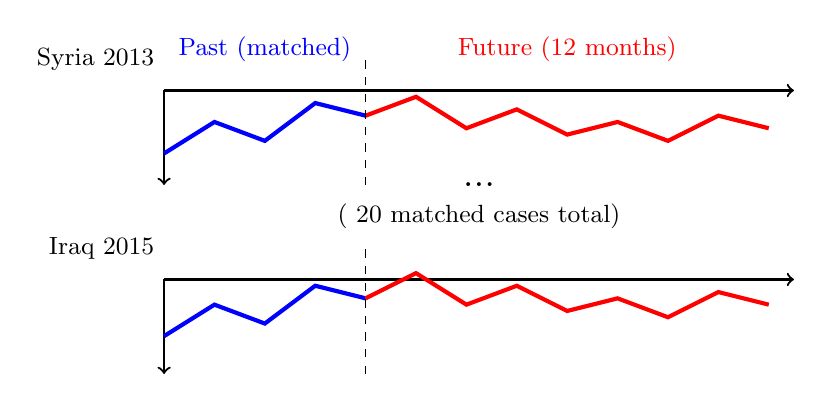
\begin{tikzpicture}[scale=0.8]
% Match 1
\node[left, font=\small] at (0,4.5) {Syria 2013};
\draw[->, thick] (0,4) -- (10,4);
\draw[->, thick] (0,4) -- (0,2.5);
% Past (similar to input)
\draw[blue, very thick, line width=1.5pt] (0,3) -- (0.8,3.5) -- (1.6,3.2) -- (2.4,3.8) -- (3.2,3.6);
% Future
\draw[red, very thick, line width=1.5pt] (3.2,3.6) -- (4,3.9) -- (4.8,3.4) -- (5.6,3.7) -- (6.4,3.3) -- (7.2,3.5) -- (8,3.2) -- (8.8,3.6) -- (9.6,3.4);
\draw[dashed] (3.2,2.5) -- (3.2,4.5);
\node[above, blue, font=\small] at (1.6,4.3) {Past (matched)};
\node[above, red, font=\small] at (6.4,4.3) {Future (12 months)};

% Match 2
\node[left, font=\small] at (0,1.5) {Iraq 2015};
\draw[->, thick] (0,1) -- (10,1);
\draw[->, thick] (0,1) -- (0,-0.5);
\draw[blue, very thick, line width=1.5pt] (0,0.1) -- (0.8,0.6) -- (1.6,0.3) -- (2.4,0.9) -- (3.2,0.7);
\draw[red, very thick, line width=1.5pt] (3.2,0.7) -- (4,1.1) -- (4.8,0.6) -- (5.6,0.9) -- (6.4,0.5) -- (7.2,0.7) -- (8,0.4) -- (8.8,0.8) -- (9.6,0.6);
\draw[dashed] (3.2,-0.5) -- (3.2,1.5);

% Ellipsis
\node at (5,2.5) {\Large ...};
\node[font=\small] at (5,2) {(~20 matched cases total)};
\end{tikzpicture}
\end{center}

\vspace{0.2cm}

For each of the $\sim$20 matches, extract the 12 months that followed

\note[item]{Step 2A: Extract futures from matched patterns}
\note[item]{We have ~20 similar historical patterns}
\note[item]{For each: Look at what happened in next 12 months}
\note[item]{Example: Syria 2013 matched our input}
\note[item]{Blue part: The pattern that matched (similar shape to input)}
\note[item]{Red part: What actually happened next (the "future")}
\note[item]{Do this for all ~20 matches}
\note[item]{Now we have ~20 different possible futures}
\note[item]{Question: Which future should we use for prediction?}
\note[item]{Can't just average - might mix escalation and de-escalation}
\note[item]{Need clustering to group similar outcomes}
\end{frame}

\begin{frame}{Shape Finder: Clustering Futures \& Making Prediction}
\textbf{Find the most common outcome}

\begin{columns}
\begin{column}{0.42\textwidth}
\textbf{Clustering Step}
\begin{enumerate}
\item Take all ~20 futures
\item Apply hierarchical clustering
\item Cut tree at optimized height
\item Result: 2--4 clusters (scenarios)
\end{enumerate}

\vspace{0.3cm}

\textbf{Prediction = Majority Cluster}
\begin{itemize}
\item Select largest cluster
\item Compute centroid (average)
\item This is the forecast
\end{itemize}

\vspace{0.3cm}

\textbf{Rationale}
\begin{itemize}
\item Most common outcome = most reliable
\item Filters outliers automatically
\item Captures consensus among matches
\end{itemize}
\end{column}
\begin{column}{0.5\textwidth}
\vspace{-7cm}
\begin{center}
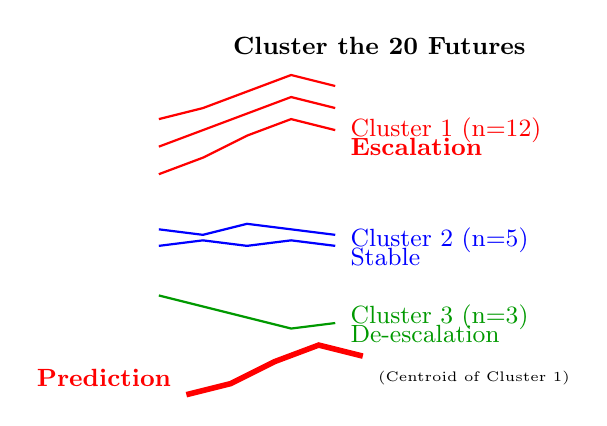
\begin{tikzpicture}[scale=0.7]
% Title
\node[above] at (4,5) {\small \textbf{Cluster the 20 Futures}};

% Three example futures - Cluster 1 (escalation)
\draw[red, thick] (0,4) -- (0.8,4.2) -- (1.6,4.5) -- (2.4,4.8) -- (3.2,4.6);
\draw[red, thick] (0,3.5) -- (0.8,3.8) -- (1.6,4.1) -- (2.4,4.4) -- (3.2,4.2);
\draw[red, thick] (0,3) -- (0.8,3.3) -- (1.6,3.7) -- (2.4,4) -- (3.2,3.8);
\node[right, red, font=\small] at (3.3,3.8) {Cluster 1 (n=12)};
\node[right, red, font=\small] at (3.3,3.5) {\textbf{Escalation}};

% Cluster 2 (stable)
\draw[blue, thick] (0,2) -- (0.8,1.9) -- (1.6,2.1) -- (2.4,2) -- (3.2,1.9);
\draw[blue, thick] (0,1.7) -- (0.8,1.8) -- (1.6,1.7) -- (2.4,1.8) -- (3.2,1.7);
\node[right, blue, font=\small] at (3.3,1.8) {Cluster 2 (n=5)};
\node[right, blue, font=\small] at (3.3,1.5) {Stable};

% Cluster 3 (de-escalation)
\draw[green!60!black, thick] (0,0.8) -- (0.8,0.6) -- (1.6,0.4) -- (2.4,0.2) -- (3.2,0.3);
\node[right, green!60!black, font=\small] at (3.3,0.4) {Cluster 3 (n=3)};
\node[right, green!60!black, font=\small] at (3.3,0.1) {De-escalation};

% Prediction (majority cluster centroid)
\draw[red, ultra thick, line width=2pt] (0.5,-1) -- (1.3,-0.8) -- (2.1,-0.4) -- (2.9,-0.1) -- (3.7,-0.3);
\node[left, red, font=\small] at (0.4,-0.7) {\textbf{Prediction}};
\node[right, font=\tiny] at (3.8,-0.7) {(Centroid of Cluster 1)};
\end{tikzpicture}
\end{center}
\end{column}
\end{columns}

\note[item]{Step 2B: Cluster futures and select prediction}
\note[item]{We have ~20 different possible futures}
\note[item]{Apply hierarchical clustering to group similar outcomes}
\note[item]{Example shown: 3 clusters emerge}
\note[item]{Cluster 1 (red): 12 cases show escalation}
\note[item]{Cluster 2 (blue): 5 cases show stability}
\note[item]{Cluster 3 (green): 3 cases show de-escalation}
\note[item]{Select majority cluster: Cluster 1 with 12 cases}
\note[item]{Compute centroid of that cluster}
\note[item]{This becomes our prediction: Escalation}
\note[item]{Rationale: Most historically common outcome}
\note[item]{Automatically filters out outliers (small clusters)}
\note[item]{Result: Risk-taking forecast that captures variability}
\end{frame}

\begin{frame}{Shape Finder: Key Advantages}

\begin{columns}
\begin{column}{0.48\textwidth}
\textbf{Methodological}
\begin{itemize}
\item \textbf{Purely autoregressive}: Uses only past fatalities
\item \textbf{No covariates}: No need for GDP, regime type, etc.
\item \textbf{Flexible}: Handles varying speeds via DTW
\item \textbf{Robust}: Clustering filters outliers
\end{itemize}

\vspace{0.5cm}

\textbf{Practical}
\begin{itemize}
\item \textbf{Fast}: Minutes, not hours
\item \textbf{Always available}: No lag for covariate updates
\end{itemize}
\end{column}
\begin{column}{0.48\textwidth}
\textbf{Performance}
\begin{itemize}
\item \textbf{Captures variability}: Predicts surges/declines
\item \textbf{Risk-taking}: Not just flat mean predictions
\item \textbf{Excels in high-complexity cases}
\end{itemize}

\vspace{0.5cm}

\textbf{Interpretability}
\begin{itemize}
\item Can cite specific historical analogues: "Trajectory similar to Syria 2012, Iraq 2015"
\item Policymakers understand the reasoning
\end{itemize}
\end{column}
\end{columns}

\note[item]{Summary of Shape Finder advantages}
\note[item]{Methodological: Pure time series approach}
\note[item]{No need to collect/update dozens of covariates}
\note[item]{DTW handles conflicts unfolding at different speeds}
\note[item]{Clustering provides robustness against outliers}
\note[item]{Practical advantages for operational use}
\note[item]{Fast: Can update forecasts daily if needed}
\note[item]{Data-light: Fatalities available immediately}
\note[item]{Performance: Key innovation is capturing variability}
\note[item]{Most models produce flat forecasts around mean}
\note[item]{Shape Finder predicts actual ups and downs}
\note[item]{Accuracy comparable to state-of-the-art (VIEWS)}
\note[item]{Interpretability: Huge advantage for policy}
\note[item]{Can explain: "Like Syria 2012" is actionable}
\note[item]{"Random forest = 87\%" is not actionable}
\note[item]{Flat inputs: If no violence in input, predict no violence}
\end{frame}



\begin{frame}{Shape Finder: Overview}
\textbf{Goal}: Forecast fatalities by finding similar historical trajectories

\begin{center}
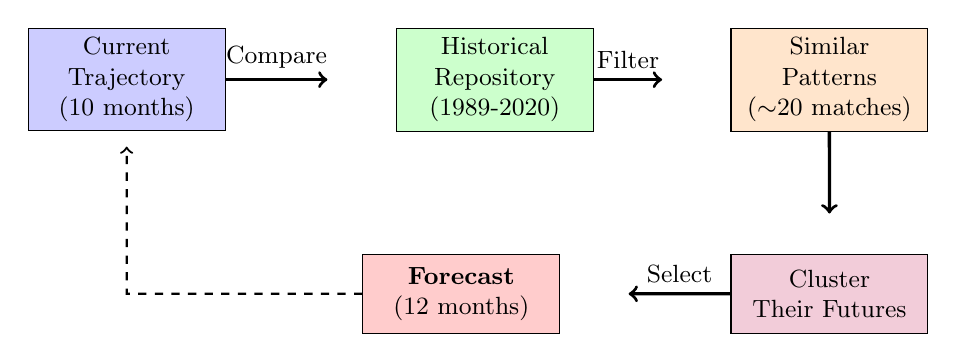
\begin{tikzpicture}[scale=0.85, every node/.style={font=\small}]
% Input
\node[draw, rectangle, fill=blue!20, minimum width=2.5cm, minimum height=1cm, align=center] (input) at (0,0) {Current\\Trajectory\\(10 months)};

% Arrow 1
\draw[->, very thick] (input) -- (3,0) node[midway, above] {Compare};

% Historical repository
\node[draw, rectangle, fill=green!20, minimum width=2.5cm, minimum height=1cm, align=center] (repo) at (5.5,0) {Historical\\Repository\\(1989-2020)};

% Arrow 2
\draw[->, very thick] (repo) -- (8,0) node[midway, above] {Filter};

% Filtered matches
\node[draw, rectangle, fill=orange!20, minimum width=2.5cm, minimum height=1cm, align=center] (matches) at (10.5,0) {Similar\\Patterns\\($\sim$20 matches)};

% Arrow down
\draw[->, very thick] (matches) -- (10.5,-2);

% Clustering
\node[draw, rectangle, fill=purple!20, minimum width=2.5cm, minimum height=1cm, align=center] (cluster) at (10.5,-3.2) {Cluster\\Their Futures};

% Arrow 3
\draw[->, very thick] (cluster) -- (7.5,-3.2) node[midway, above] {Select};

% Prediction
\node[draw, rectangle, fill=red!20, minimum width=2.5cm, minimum height=1cm, align=center] (pred) at (5,-3.2) {\textbf{Forecast}\\(12 months)};

% Back to start indication
\draw[->, dashed, thick] (pred) -- (0,-3.2) -- (0,-1);
\end{tikzpicture}
\end{center}

\vspace{0.3cm}


\note[item]{Shape Finder: Pattern-based forecasting from Schincariol et al. 2025}
\note[item]{Overview of the complete algorithm before diving into details}
\note[item]{Start with current 10-month trajectory - what we observe now}
\note[item]{Compare to comprehensive historical repository - all countries 1989-2020}
\note[item]{Filter to find $\sim$20 most similar historical patterns}
\note[item]{Look at what happened after those similar patterns}
\note[item]{Cluster those futures to find most common outcome}
\note[item]{Make prediction based on majority cluster}
\note[item]{This is a risk-taking model - captures variability}
\note[item]{Complements risk-averse models like VIEWS}
\end{frame}



%\begin{frame}
%\begin{center}
%\includegraphics[width=0.85\textwidth]{Figs/method1.png}
%\end{center}
%\end{frame}
%
%\begin{frame}
%\begin{center}
%\includegraphics[width=0.85\textwidth]{Figs/method2.png}
%\end{center}
%\end{frame}

% ====================
% PART 5: RESULTS - FIVE QUESTIONS
% ====================

\section{Results: Four Questions}

\begin{frame}{Four Research Questions}
\Large
\begin{enumerate}
\item Do conflict sequences repeat?
\item Do conflict sequences repeat across space and time?
\item Do similar patterns predict similar futures?
\item Can we model richer shapes?
\end{enumerate}

\note[item]{Structure results around four questions}
\note[item]{Each tests a key hypothesis}
\note[item]{Build from basic (do patterns exist?) to applied (can we forecast?)}
\note[item]{This also tells story of the research program}
\note[item]{Let's go through each systematically...}
\end{frame}




\begin{frame}{Q1: Do Conflict Sequences Repeat?}

\begin{columns}
\begin{column}{0.5\textwidth}
\includegraphics[width=\textwidth]{Figs/General_shape_mot1.png}
\begin{center}\textbf{Motif 1: M-shaped}\end{center}

\vspace{0.3cm}

\end{column}
\begin{column}{0.5\textwidth}
\includegraphics[width=\textwidth]{Figs/General_shape_mot2.png}
\begin{center}\textbf{Motif 2: Delayed Escalation}\end{center}

\vspace{0.3cm}

\end{column}
\end{columns}

\note[item]{What do the actual patterns look like?}
\note[item]{Motif 1 (M-shaped): Multiple peaks with regular intervals}
\note[item]{Interpretation: Repeated mobilization-demobilization cycles}
\note[item]{Could reflect: Failed peace talks, seasonal patterns, tactical pauses}
\note[item]{10-month interval: Time to rearm, recruit, regroup}
\note[item]{Motif 2 (Delayed): Long stable period then sudden jump}
\note[item]{Interpretation: Underlying tensions building invisibly}
\note[item]{Then trigger event causes rapid escalation}
\note[item]{Early warning value: 12-month plateau before surge}
\note[item]{If current conflict matches this pattern $\rightarrow$ prepare for escalation}
\note[item]{These aren't the only motifs, but most frequent}
\note[item]{Point: Patterns are interpretable, recognizable}
\end{frame}


\begin{frame}{Q1: Do Conflict Sequences Repeat?}

Groups similar sequences together (combine if $d_{dtw}(s_1,s_2) < threshold$) and plot distribution. 


\begin{columns}
\begin{column}{0.33\textwidth}
\includegraphics[width=\textwidth]{Figs/Distrib_matches_earth.png}
\begin{center}\small Earthquakes\end{center}

\vspace{0.3cm}

\includegraphics[width=\textwidth]{Figs/Distrib_matches_stock.png}
\begin{center}\small Stock Market\end{center}
\end{column}
\begin{column}{0.33\textwidth}
\includegraphics[width=\textwidth]{Figs/Distrib_matches_rainfall.png}
\begin{center}\small Rainfall\end{center}

\vspace{0.3cm}

\includegraphics[width=\textwidth]{Figs/Distrib_matches_temp.png}
\begin{center}\small Temperature\end{center}
\end{column}
\begin{column}{0.33\textwidth}
\includegraphics[width=\textwidth]{Figs/Distrib_matches.png}
\begin{center}\small \textbf{Conflict}\end{center}

\vspace{0.3cm}

\includegraphics[width=\textwidth]{Figs/Distrib_matches_white.png}
\begin{center}\small White Noise\end{center}
\end{column}
\end{columns}


\note[item]{Comparison across domains using identical methodology}
\note[item]{Earthquakes: Aftershock sequences, recurring patterns - similar to conflict}
\note[item]{Rainfall: Seasonal cycles, recurring patterns - similar to conflict}
\note[item]{Stock markets: More random, efficient market hypothesis - different from conflict}
\note[item]{Temperature: Strong regular cycles - somewhat similar}
\note[item]{White noise: Flat distribution - very different from conflict}
\note[item]{Key insight: Conflicts cluster with natural recurrent processes}
\note[item]{Not like random or efficient systems}
\note[item]{Suggests underlying generative mechanisms similar to natural systems}
\note[item]{Reinforces: Pattern-based approach is appropriate}
\end{frame}

\begin{frame}{Q2: Do Motifs Generalize Across Space and Time?}

\begin{center}
\includegraphics[width=0.6\textheight]{Figs/Heatmap_Scale.png}
\end{center}


\note[item]{Question 2: Are patterns universal or context-specific?}
\note[item]{Test: Compare pattern distributions across different categories}
\note[item]{Heatmap shows: Conditional probability ratios}
\note[item]{If similar patterns share same motif more than chance $\rightarrow$ >1}
\note[item]{Diagonal dominance: Yes, patterns consistent within categories}
\note[item]{But also: Off-diagonal elements present}
\note[item]{Meaning: Same motifs appear in small and large conflicts}
\note[item]{M-shaped pattern in both 10-death and 1000-death conflicts}
\note[item]{This is evidence for universality}
\note[item]{Scale doesn't determine pattern type}
\note[item]{Next: Geography...}
\end{frame}

\begin{frame}{Q2: Do They Travel Across Space and Time?}
\begin{columns}
\begin{column}{0.5\textwidth}
\includegraphics[width=\textwidth]{Figs/Heatmap_Region.png}
\begin{center}\textbf{Across Regions}\end{center}

\end{column}
\begin{column}{0.5\textwidth}
\includegraphics[width=\textwidth]{Figs/Heatmap_Decade.png}
\begin{center}\textbf{Across Decades}\end{center}
\end{column}
\end{columns}

\note[item]{Geographic test: Do African patterns differ from Asian patterns?}
\note[item]{Heatmap: Some regional clustering, but substantial overlap}
\note[item]{Same motifs appear in Syria and Colombia}
\note[item]{In Afghanistan and Nigeria}
\note[item]{Despite totally different: cultures, resources, actors, grievances}
\note[item]{Suggests: Common generative processes}
\note[item]{Temporal test: 1990s vs 2010s}
\note[item]{If patterns were data quality artifacts $\rightarrow$ would change over time}
\note[item]{(Data quality improved substantially 1990s$\rightarrow$2010s)}
\note[item]{But patterns stable across decades}
\note[item]{Strong evidence: Patterns are real, not measurement artifacts}
\note[item]{Universality is remarkable - enables cross-context learning}
\end{frame}

\begin{frame}{Q3: Do Patterns Predict The Future?}


 Do Similar Patterns Predict Similar Futures?
\begin{center}
\includegraphics[width=0.55\textwidth]{Figs/h_1.png}
\end{center}


\note[item]{Question 3: Critical validation of the entire approach}
\note[item]{If patterns are meaningful for forecasting, then:}
\note[item]{More similar patterns $\rightarrow$ more similar futures}
\note[item]{X-axis: Dissimilarity between current patterns (DTW distance)}
\note[item]{Y-axis: Standard deviation of subsequent developments}
\note[item]{Clear inverse relationship: Lower D $\rightarrow$ Lower $\sigma$}
\note[item]{When current trajectories are very similar (low dissimilarity)}
\note[item]{Their futures are consistent (low variability)}
\note[item]{When current trajectories differ (high dissimilarity)}
\note[item]{Their futures are unpredictable (high variability)}
\note[item]{This is exactly what we'd expect if patterns carry information}
\note[item]{Validates: Using pattern similarity for forecasting}
\note[item]{Not just correlation - this is mechanism validation}
\end{frame}



\begin{frame}{Q3: Do Patterns Predict The Future?}
Test set: fatalities 2022--2023\\
Learning set: Fatalities 1989--2020
\begin{center}
\includegraphics[width=0.95\textwidth]{Figs/results1.png}
\end{center}
\end{frame}

\begin{frame}{Q3: Do Patterns Predict The Future?}
\begin{center}
\includegraphics[width=0.95\textwidth]{Figs/sampleResults.png}
\end{center}
\end{frame}


\begin{frame}{Q3: Do Patterns Predict The Future?}
Protest patterns $\rightarrow$  Future protests

\begin{columns}
\begin{column}{0.5\textwidth}
\begin{center}
\includegraphics[width=0.95\textwidth]{Figs/indiaProtests.jpg}
\end{center}
\end{column}
\begin{column}{0.5\textwidth}
\begin{center}
\includegraphics[width=0.95\textwidth]{Figs/protestsResults1.jpg}
\end{center}
\end{column}
\end{columns}

\end{frame}



\begin{frame}{Q3: Do Patterns Predict The Future?}
Protest patterns  $\rightarrow$ future conflict

\includegraphics[width=0.95\textwidth]{Figs/protestPatternsEscalation2.png}

\end{frame}


\begin{frame}{Q3: Do Patterns Predict The Future?}
Protest patterns  $\rightarrow$  future one-sided violence

\includegraphics[height=0.85\textheight]{Figs/protestsOneSidedViolence3.png}

\end{frame}

\begin{frame}{Q3: Do Patterns Predict The Future?}
Migration patterns $\rightarrow$  future migration

\begin{columns}
\begin{column}{0.5\textwidth}
\begin{center}
\includegraphics[width=1\textwidth]{Figs/migration1.png}
\end{center}
\end{column}
\begin{column}{0.5\textwidth}
\begin{center}
\includegraphics[width=1\textwidth]{Figs/migration2.png}
\end{center}
\end{column}
\end{columns}

\end{frame}




\begin{frame}{Q3: Do Patterns Predict The Future?}
Stock market  $\rightarrow$  Rockets

\includegraphics[width=0.95\textwidth]{Figs/rockets1.png}

\end{frame}


\begin{frame}{Q5: Can We Model Richer 3D Shapes?}
\textbf{Extension}: Incorporate spatial dimension alongside temporal

\begin{center}
\includegraphics[width=0.9\textwidth]{Figs/Data_process.JPG}
\end{center}

\textbf{source}: Schincariol 2026

\note[item]{Question 5: Can we go beyond 1D time series?}
\note[item]{Conflicts occur in space AND time}
\note[item]{Violence doesn't just escalate, it spreads geographically}
\note[item]{Step 1: Identify active cells in 2D geographic grid}
\note[item]{Step 2: Extract connected components - "molecules" of conflict}
\note[item]{3D visualization: Longitude, latitude, time}
\note[item]{Darker intensity = more fatalities}
\note[item]{Step 3: Convert to density cube}
\note[item]{Each dimension normalized, conflict intensity as density}
\note[item]{Now can compute geometric similarity (Mahalanobis distance)}
\note[item]{Find conflicts with similar spatio-temporal shapes}
\note[item]{Next slide: What this enables...}
\end{frame}


% ====================
% PART 6: THE RESEARCH PROGRAM
% ====================
% ====================
% PART 7: APPLICATIONS & FUTURE
% ====================

\section{Applications \& Future Directions}

\begin{frame}{Live Operational Forecasting}
\textbf{Operational system}: Monthly forecasts 6 months ahead, all countries

\begin{columns}
\begin{column}{0.5\textwidth}
\textbf{Performance (2024)}
\begin{itemize}
\item Forecasts for Feb-July 2024
\item Validated against observed fatalities
\item Compared to ViEWS and ConflictForecast
\end{itemize}

\vspace{0.5cm}

\textbf{Results}
\begin{itemize}
\item Outperformed ViEWS in 75\% of cases
\item Outperformed ConflictForecast in 70-74\%
\item Best performance in high-intensity conflicts
\end{itemize}
\end{column}


\begin{column}{0.5\textwidth}
\textbf{Advantages}
\begin{itemize}
\item Timing specificity
\item Interpretable (shows historical analogs)
\item Minimal data requirements
\item Fast computation
\end{itemize}

\vspace{0.5cm}

\textbf{Use Cases}
\begin{itemize}
\item Humanitarian early warning
\item Diplomatic planning
\item Resource allocation
\item Risk assessment
\end{itemize}
\end{column}
\end{columns}

\note[item]{Not just retrospective - operational system}
\note[item]{Generates forecasts monthly for all countries}
\note[item]{6-month ahead predictions of fatality counts}
\note[item]{2024 test: Forecasted Feb-July, compared to what happened}
\note[item]{Benchmarked against two leading systems}
\note[item]{ViEWS: Uppsala University system, covariate-rich}
\note[item]{ConflictForecast: Another operational system}
\note[item]{Our system outperformed in 70-75\% of cases}
\note[item]{Particularly strong for high-intensity conflicts}
\note[item]{These are the cases that matter most for policy}
\note[item]{Advantages: Interpretable - can explain why}
\note[item]{"Forecast based on similarity to Syria 2013"}
\note[item]{Minimal data - just need fatality time series}
\note[item]{Fast - no need to update 50 covariates monthly}
\note[item]{Use cases: Multiple applications}
\end{frame}

\begin{frame}{Limitations}
\textbf{Important caveats}

\begin{columns}
\begin{column}{0.5\textwidth}
\textbf{Data Limitations}
\begin{itemize}
\item UCDP coverage varies
\item Remote conflicts under-reported
\item Measurement error in fatalities
\end{itemize}

\vspace{0.5cm}

\textbf{Methodological Challenges}
\begin{itemize}
\item Window length choice
\item Normalization decisions
\item Number of clusters (k)
\item Distance metric choice
\end{itemize}
\end{column}
\begin{column}{0.5\textwidth}
\textbf{External Validity}
\begin{itemize}
\item Low-visibility conflicts
\item Novel conflict types
\item Unprecedented escalations
\item Structural breaks
\end{itemize}

\vspace{0.5cm}

\textbf{Forecast Limitations}
\begin{itemize}
\item Accuracy degrades with horizon
\item Uncertainty quantification challenging
\item Rare events hard to predict
\item No causal identification
\end{itemize}
\end{column}
\end{columns}


\note[item]{Important to acknowledge limitations}
\note[item]{Data: UCDP is best available but imperfect}
\note[item]{Coverage better in some regions (Middle East) than others (Central Africa)}
\note[item]{Fatality counts have error bars - exact numbers uncertain}
\note[item]{How to define "episode"? When does conflict start/end?}
\note[item]{Methodological: Several choices affect results}
\note[item]{Window length: 12 vs 24 vs 36 months - which is right?}
\note[item]{We test robustness, but choices matter}
\note[item]{K in clustering: How many motifs? Data-driven but subjective}
\note[item]{External validity: Works for documented conflicts}
\note[item]{But what about totally novel conflicts? Unprecedented events?}
\note[item]{Arab Spring wasn't predictable from past patterns}
\note[item]{Forecasting: Accuracy drops as horizon extends}
\note[item]{6 months ahead: good. 2 years ahead: poor}
\note[item]{This is prediction, not causal inference}
\note[item]{Can't say intervention X will reduce violence Y percent}
\note[item]{Can say: trajectory resembles historical pattern Z}
\end{frame}

\begin{frame}{Irreducible Sources of Error}
\textbf{Why we can't achieve perfect forecasts} (Schrodt 2018)

\begin{columns}
\begin{column}{0.5\textwidth}
\textbf{Model \& Data Issues}
\begin{enumerate}
\item \textbf{Specification error}

\vspace{0.2cm}

\item \textbf{Measurement error}
\end{enumerate}
\end{column}
\begin{column}{0.5\textwidth}
\textbf{Fundamental Limits}
\begin{enumerate}
\setcounter{enumi}{2}
\item \textbf{Quasi-random structural error}
\begin{itemize}
\item Complex systems
\item Chaotic systems 
\end{itemize}

\vspace{0.2cm}

\item \textbf{Rational randomness}
\begin{itemize}
\item Mixed strategies in zero-sum games
\item Strategic unpredictability
\end{itemize}
\end{enumerate}
\end{column}
\end{columns}

\note[item]{Critical acknowledgment: Perfect prediction is impossible}
\note[item]{Not just practical limits, but theoretical ones}
\note[item]{Based on Schrodt's taxonomy of irreducible errors}
\note[item]{1. Specification error: Fundamental problem}
\note[item]{Can't include every variable that matters}
\note[item]{Individual psychology, weather, unobserved negotiations}
\note[item]{Model is always simplified version of reality}
\note[item]{2. Measurement error: Pervasive in conflict data}
\note[item]{Fatality counts uncertain, event coding subjective}
\note[item]{Rural areas less documented than urban}
\note[item]{Government sources vs rebel sources disagree}
\note[item]{Error propagates through models}
\note[item]{3. Quasi-random structural: Complex systems}
\note[item]{Small changes $\rightarrow$ large effects (butterfly effect)}
\note[item]{Conflicts involve many interacting agents}
\note[item]{Produces effective randomness even if deterministic}
\note[item]{4. Rational randomness: Game theory insight}
\note[item]{In zero-sum games, predictability is weakness}
\note[item]{Optimal strategy is mixed (random)}
\note[item]{Military tactics deliberately unpredictable}
\note[item]{Some conflicts strategic - inherently random}
\end{frame}

\begin{frame}{Irreducible Sources of Error (cont.)}
\textbf{Human and policy factors}

\begin{columns}
\begin{column}{0.5\textwidth}
\begin{enumerate}
\setcounter{enumi}{4}
\item \textbf{Individual randomness}
\begin{itemize}
\item Free will and individual agency
\item Unpredictable decisions by leaders
\item Idiosyncratic factors
\end{itemize}

\vspace{0.4cm}

\item \textbf{Effective policy response}
\begin{itemize}
\item Successful prevention = wrong forecast
\item Model predicts escalation
\item Policy intervenes, prevents it
\item Model appears to have "failed"
\end{itemize}
\end{enumerate}
\end{column}
\begin{column}{0.5\textwidth}
\begin{enumerate}
\setcounter{enumi}{6}
\item \textbf{Natural phenomena}
\begin{itemize}
\item Exogenous shocks
\item Example: 2004 tsunami $\rightarrow$ reduced Aceh conflict
\item Unpredictable events with large effects
\end{itemize}
\end{enumerate}

\vspace{0.5cm}

\begin{center}
\textbf{The Forecasting "Speed Limit"}

\vspace{0.3cm}

\Large
\highlight{$\sim$80-85\% accuracy ceiling}

\vspace{0.3cm}

\normalsize
Convergent finding across projects\\
and methodologies
\end{center}
\end{column}
\end{columns}

\note[item]{Continuation: Three more irreducible sources}
\note[item]{5. Arational randomness: The "free will" problem}
\note[item]{Leaders make unexpected decisions}
\note[item]{Putin's Ukraine invasion timing surprised many}
\note[item]{Individual psychology matters but unpredictable}
\note[item]{Not in our models, can't be}
\note[item]{6. Effective policy response: Paradox of prevention}
\note[item]{This is actually a GOOD thing but looks bad}
\note[item]{Model says: "High risk of escalation next month"}
\note[item]{UN intervenes, deploys peacekeepers}
\note[item]{Escalation prevented - model was "wrong"}
\note[item]{But model was useful! Enabled prevention}
\note[item]{Success looks like failure in retrospective analysis}
\note[item]{7. Natural phenomena: Truly exogenous shocks}
\note[item]{2004 tsunami: Devastated Aceh}
\note[item]{Both government and GAM rebel forces weakened}
\note[item]{Led to peace process - totally unpredicted}
\note[item]{Earthquakes, floods, pandemics affect conflicts}
\note[item]{Can't predict these, so can't predict their effects}
\note[item]{Bottom line: Speed limit around 80-85\%}
\note[item]{This finding remarkably consistent}
\note[item]{ViEWS, ConflictForecast, ICEWS, our work: all similar}
\note[item]{Different methods, same ceiling}
\note[item]{Suggests fundamental limit, not methodological}
\note[item]{Implies: Don't oversell forecasting}
\note[item]{But 80\% is still very useful! Much better than 50\%}
\end{frame}

\begin{frame}{Future Directions}
\textbf{Next steps for the research program}

\begin{itemize}
\item Deep learning
\item Onset prediction
\item Theory Development
\end{itemize}
\end{frame}

\begin{frame}{Broader Implications}

\begin{itemize}
\item Forecasting is underused in the social sciences
\item Pattern recognition is almost never used in social science
\item Interpretability matters: patterns are more intuitive than black boxes
\item Temporal structure can substitute for expensive covariate collection
\end{itemize}

\vspace{0.5cm}

\begin{itemize}
\item Conflicts are somewhat predictable
\item Focus on dynamics, not just drivers
\end{itemize}

\note[item]{Broader lessons beyond this specific application}
\note[item]{For stats: Pattern methods underused in social science}
\note[item]{Economics, sociology focus on regression}
\note[item]{But many social processes are temporal patterns}
\note[item]{DTW, matrix profiles developed for CS, engineering}
\note[item]{Social scientists should adopt these tools}
\note[item]{Non-stationarity: Usually treated as problem to fix}
\note[item]{But escalation IS non-stationary - that's what we want to model!}
\note[item]{Don't difference it away, study the shape}
\note[item]{Interpretability: Critical for policy application}
\note[item]{"Random forest says 87\%" - not actionable}
\note[item]{"Trajectory matches Syria 2013" - actionable}
\note[item]{Temporal data cheaper than covariates}
\note[item]{Don't need to measure GDP, regime type monthly}
\note[item]{Just need event counts}
\note[item]{For conflict studies: Rethink what's knowable}
\note[item]{"Conflicts too complex to predict" - not true!}
\note[item]{Focus on HOW they evolve, not just WHY they start}
\note[item]{Can we bridge prediction and explanation? Yes}
\end{frame}
%
%

\begin{frame}


\vspace{1cm}

\begin{figure}
\includegraphics[width=0.7\textwidth]{Figs/paceLogo.png}
\end{figure}

\vspace{1cm}

\normalsize
Thomas Chadefaux\\
Trinity College Dublin\\
\texttt{thomas.chadefaux@tcd.ie}
\end{frame}

\begin{frame}[allowframebreaks]{References}
\footnotesize
\begin{itemize}
\item Lu, C., \& Chadefaux, T. (2026). Structured Pixels. \textit{HICSS}.
\item Cao, J., \& Chadefaux, T. Dynamic Synthetic Controls (2025). \textit{Political Analysis}.
\item Xue, Y., Schincariol, T., Chadefaux, T., \& Groen, D. (2025). Forecasting conflict events. \textit{Sci. Rep.}
\item Wu, S., Luo, X., Liu, J., \& Deng, Y. (2025). Knowledge distillation with adapted weight. \textit{Statistics}.
\item Han, J. (2025). How China's Multilateral Engagement Shapes Threat Perception amid Rising Authoritarianism. \textit{J. Contemp. China}.
\item Schincariol, T., Frank, H., \& Chadefaux, T. Accounting for variability in conflict dynamics: A pattern-based predictive model (2025). \textit{J. Peace Res.}
\item Chadefaux, T. (2024). Automated pattern recognition for conflict. \textit{J. Comput. Sci.}
\item Hegre et al., VIEWS Prediction Challenge (2024). \textit{J. Peace Res.}
\item Schincariol, T., \& Chadefaux, T. Migration patterns in migration flows (2024). \textit{J. Forecasting}.
\item Schincariol, T., Frank, H., \& Chadefaux, T. Leveraging temporal patterns (2024). \textit{IAPR Working Papers} (accepted).
\item Crisman-Cox, C., \& Park, Y. (2024). Remittances, terrorism, and democracy. \textit{Conflict Manage. Peace Sci.}
\item Jung, Y. S., \& Park, Y. (2024). US--China trade disputes. \textit{Soc. Sci. Q.}
\item Akeweje, E., \& Zhang, M. (2024). Learning mixtures of Gaussian processes. \textit{ICML}.
\end{itemize}
\end{frame}

\end{document}
